% Copyright 2026 The terCAD team. All rights reserved.
% Use of this content is governed by a CC BY-NC-ND 4.0 license that can be found in the LICENSE file.

Few mobile projects start from scratch. Most grow on top of something that already works, such
as a website, a back-office system, or in our case, a browser game that has cultivated its
community over many years. The challenge is not to invent new rules, but rather to carry the
existing experience over to a pocket-sized device without breaking what players already know and
love.

\paragraph{Project Assumption} Liga of Heroes (\href{https://fantasyland.ru}{fantasyland.ru}) is
played in a desktop browser. Its pages are designed for wide screens and mice with frames, small
tables, pop-up windows, and hover hints. The text is encoded in Windows-1251, and the entire
game state (the hero, the location, and the fight) is stored on the server. Meanwhile, players
spend their day with phones in their hands. They want to make a move on the map, respond in the
chat, or check a fight while away from a computer. The assumption is simple: \emph{A native
client that keeps the game rules on the server but adapts its interface to a touchscreen will
allow players to stay in the game wherever they are}.

\begin{figure}[h]
  \centering
  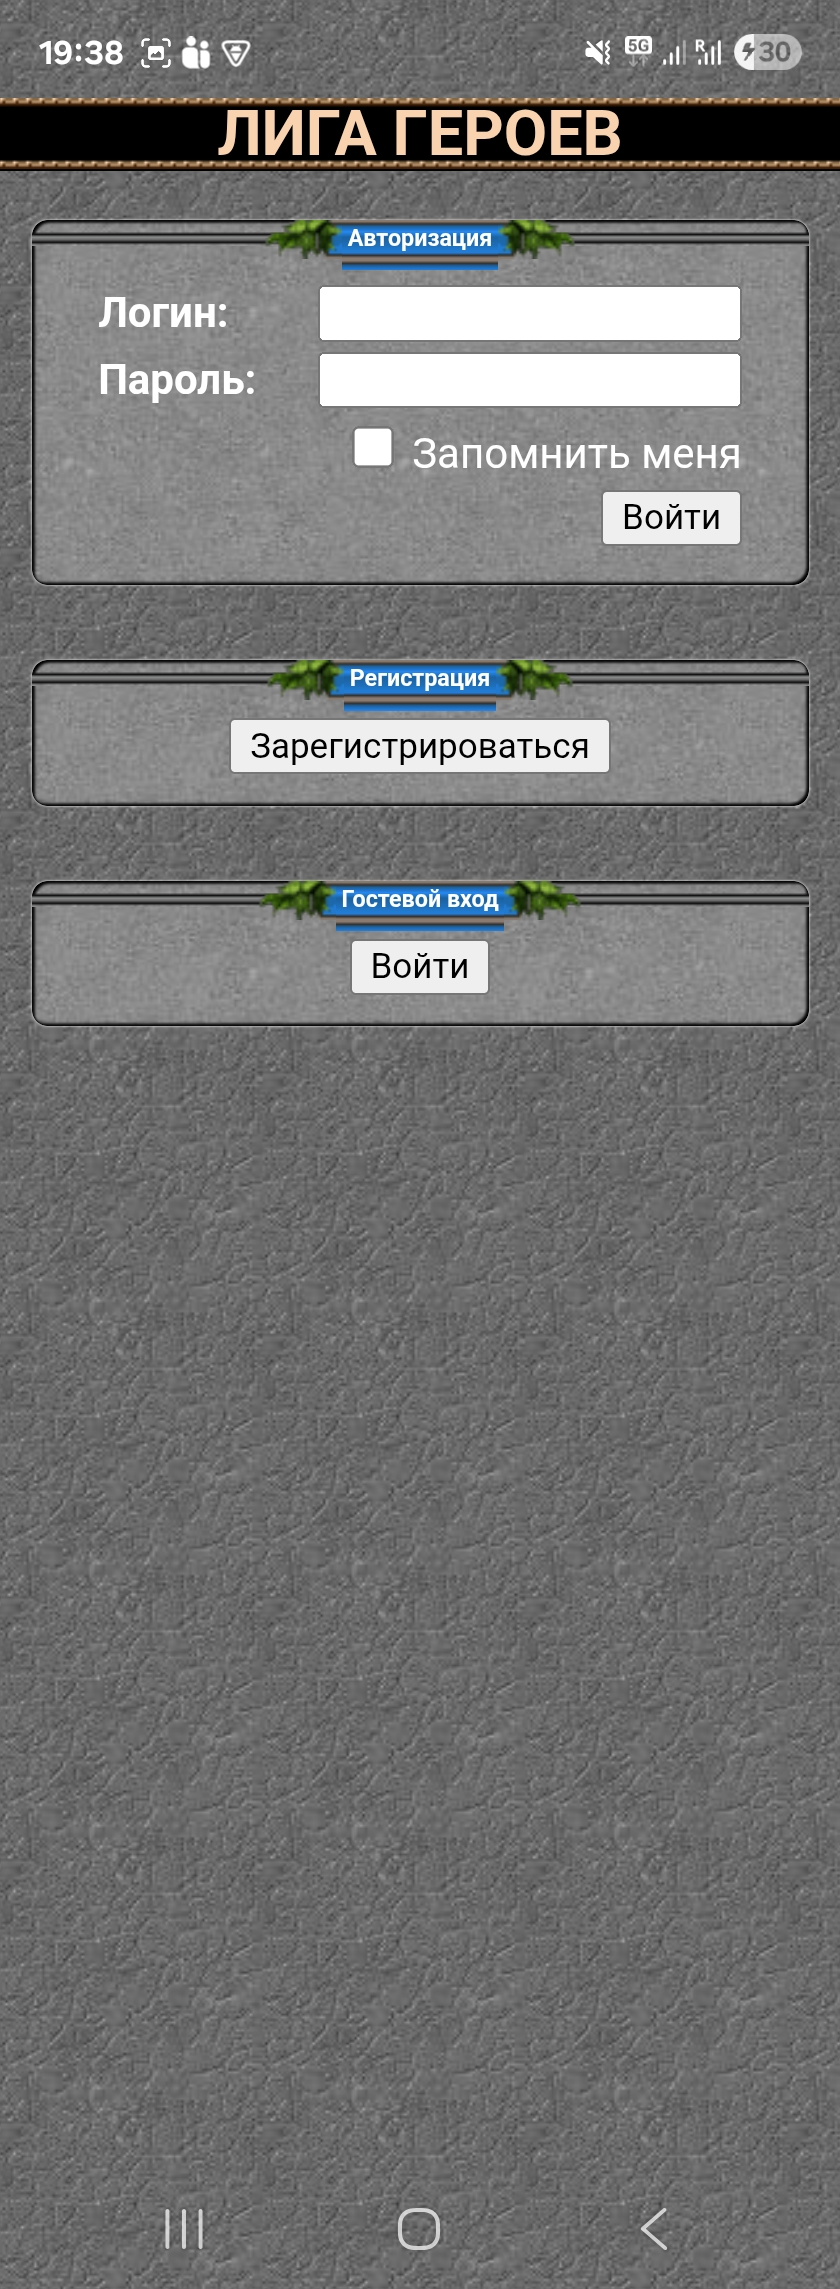
\includegraphics[width=0.24\textwidth]{../design-flow/login.jpg}\hfill
  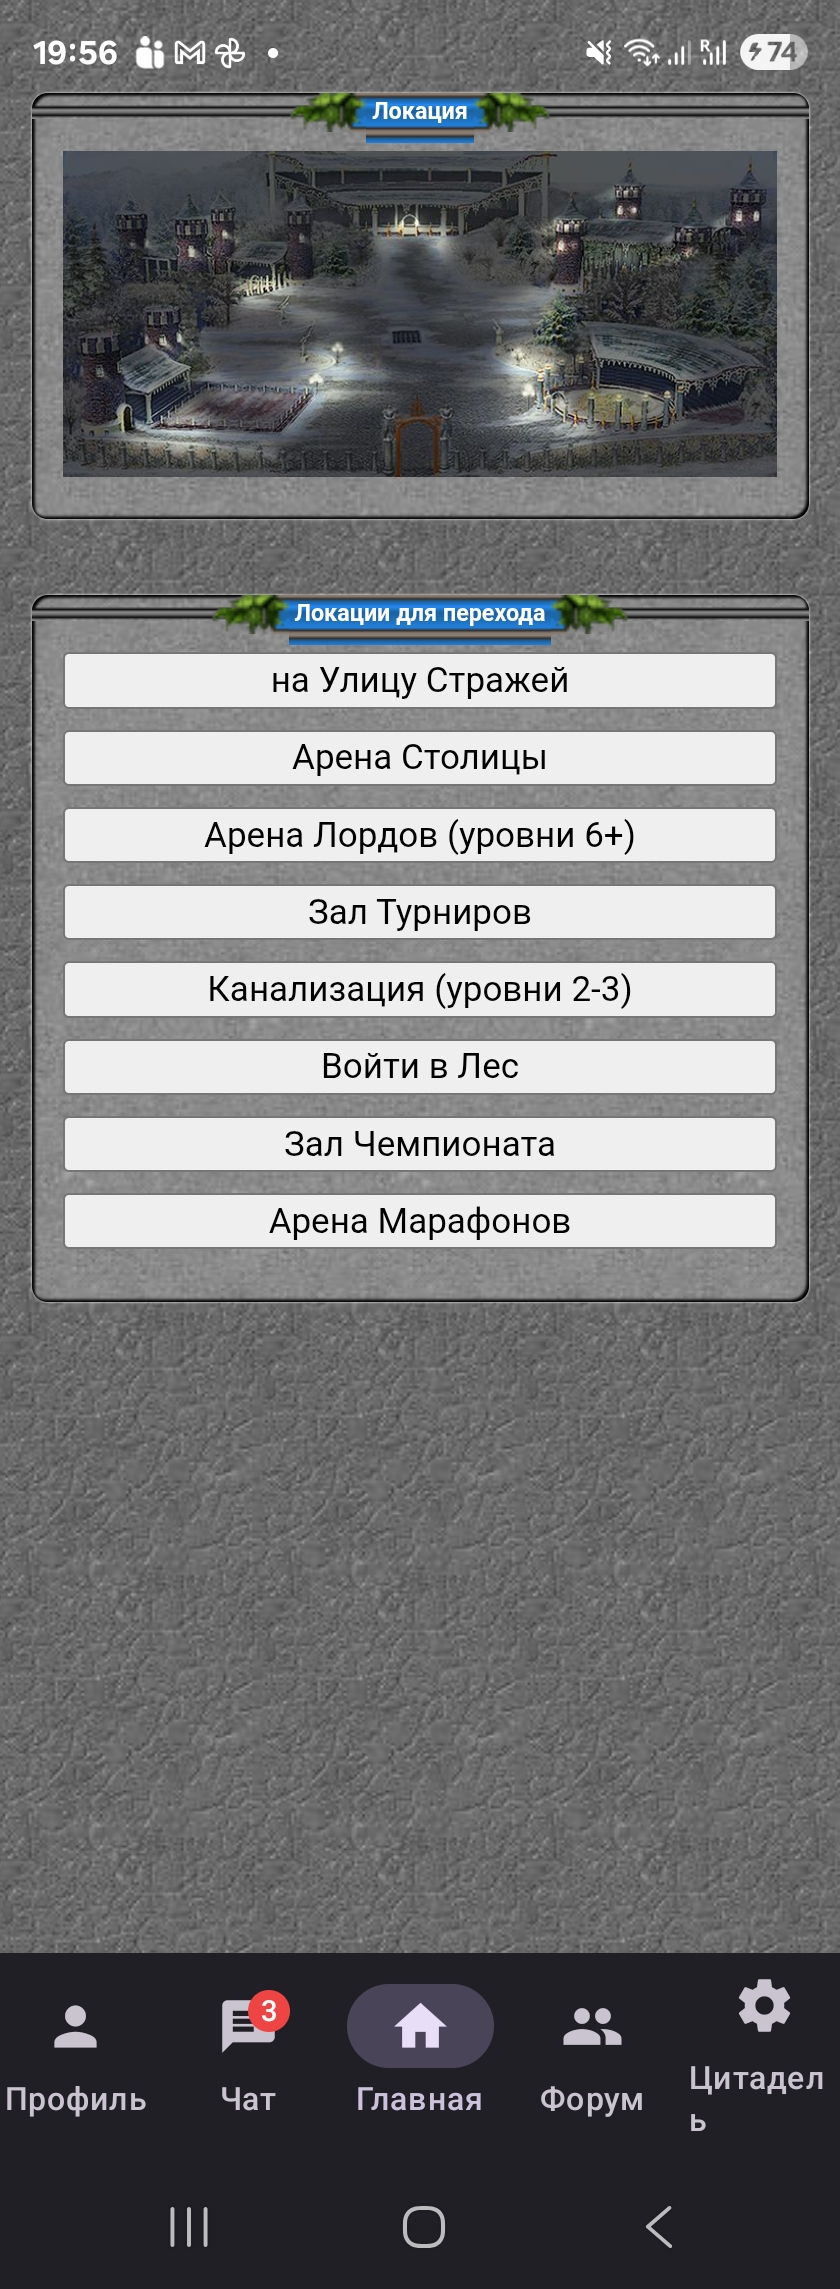
\includegraphics[width=0.24\textwidth]{../design-flow/movements.jpg}\hfill
  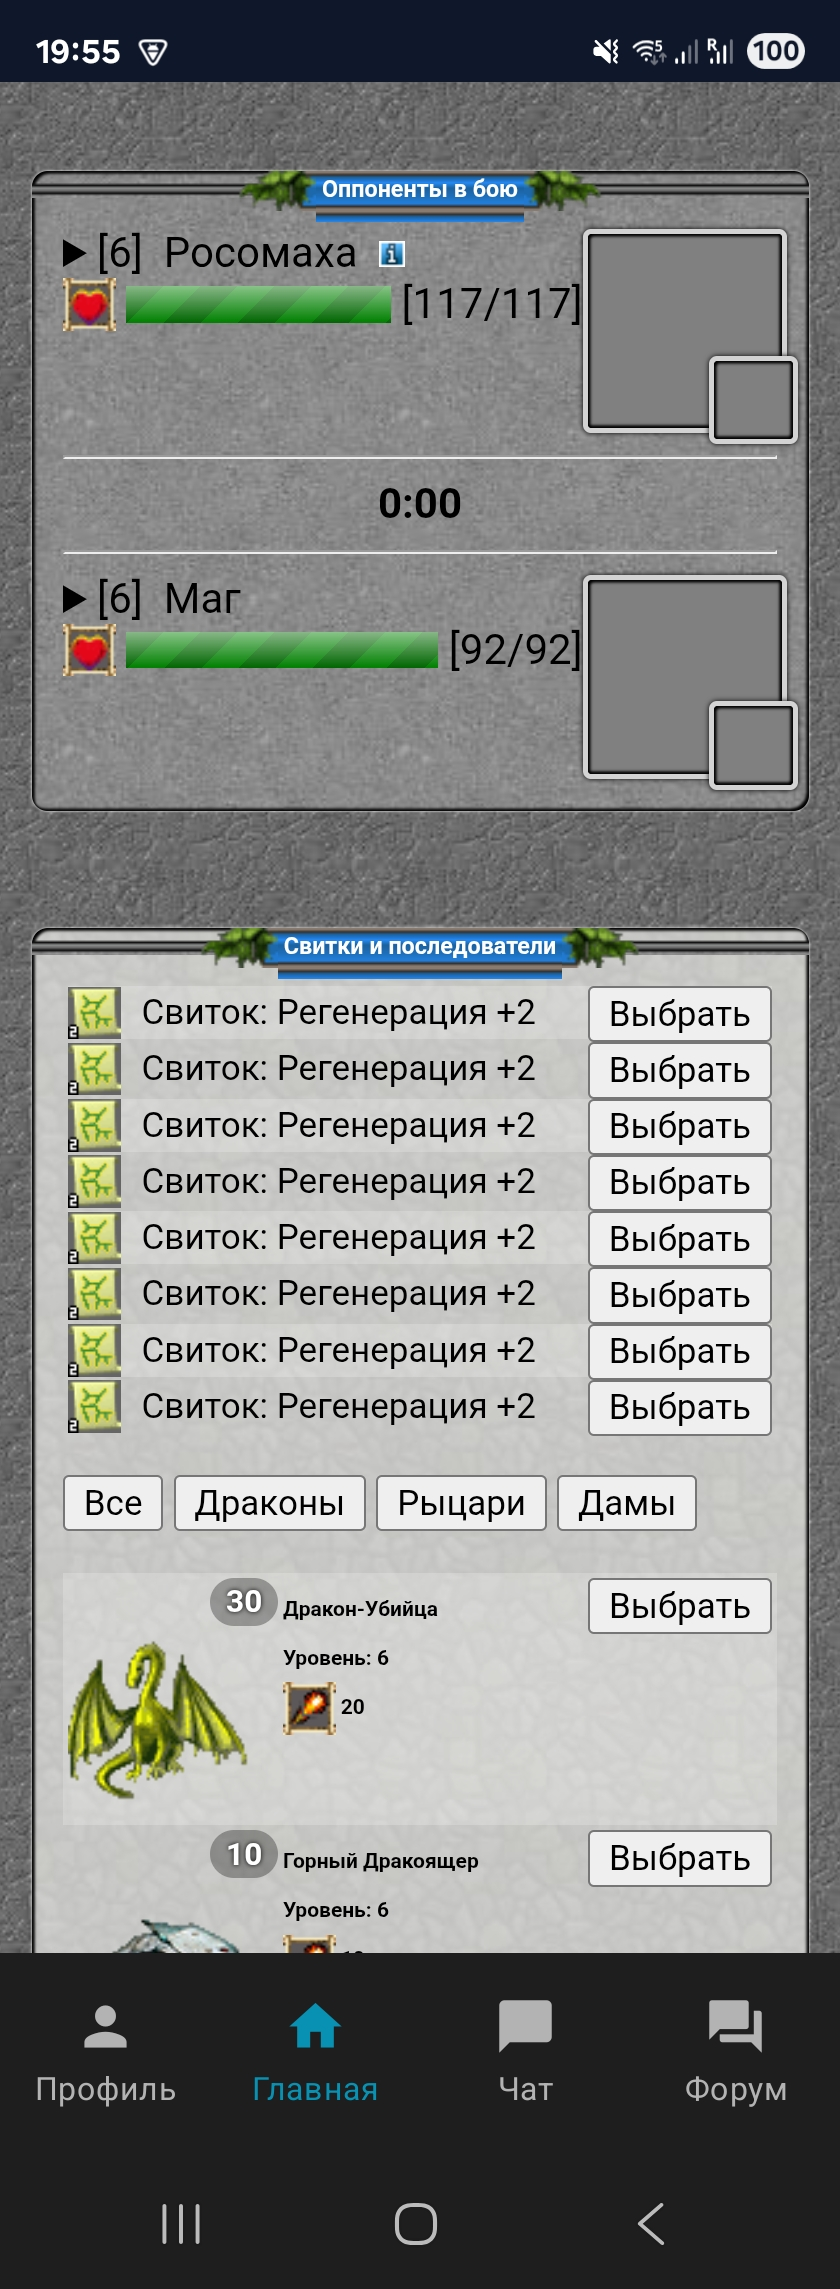
\includegraphics[width=0.24\textwidth]{../design-flow/fight_2.jpg}\hfill
  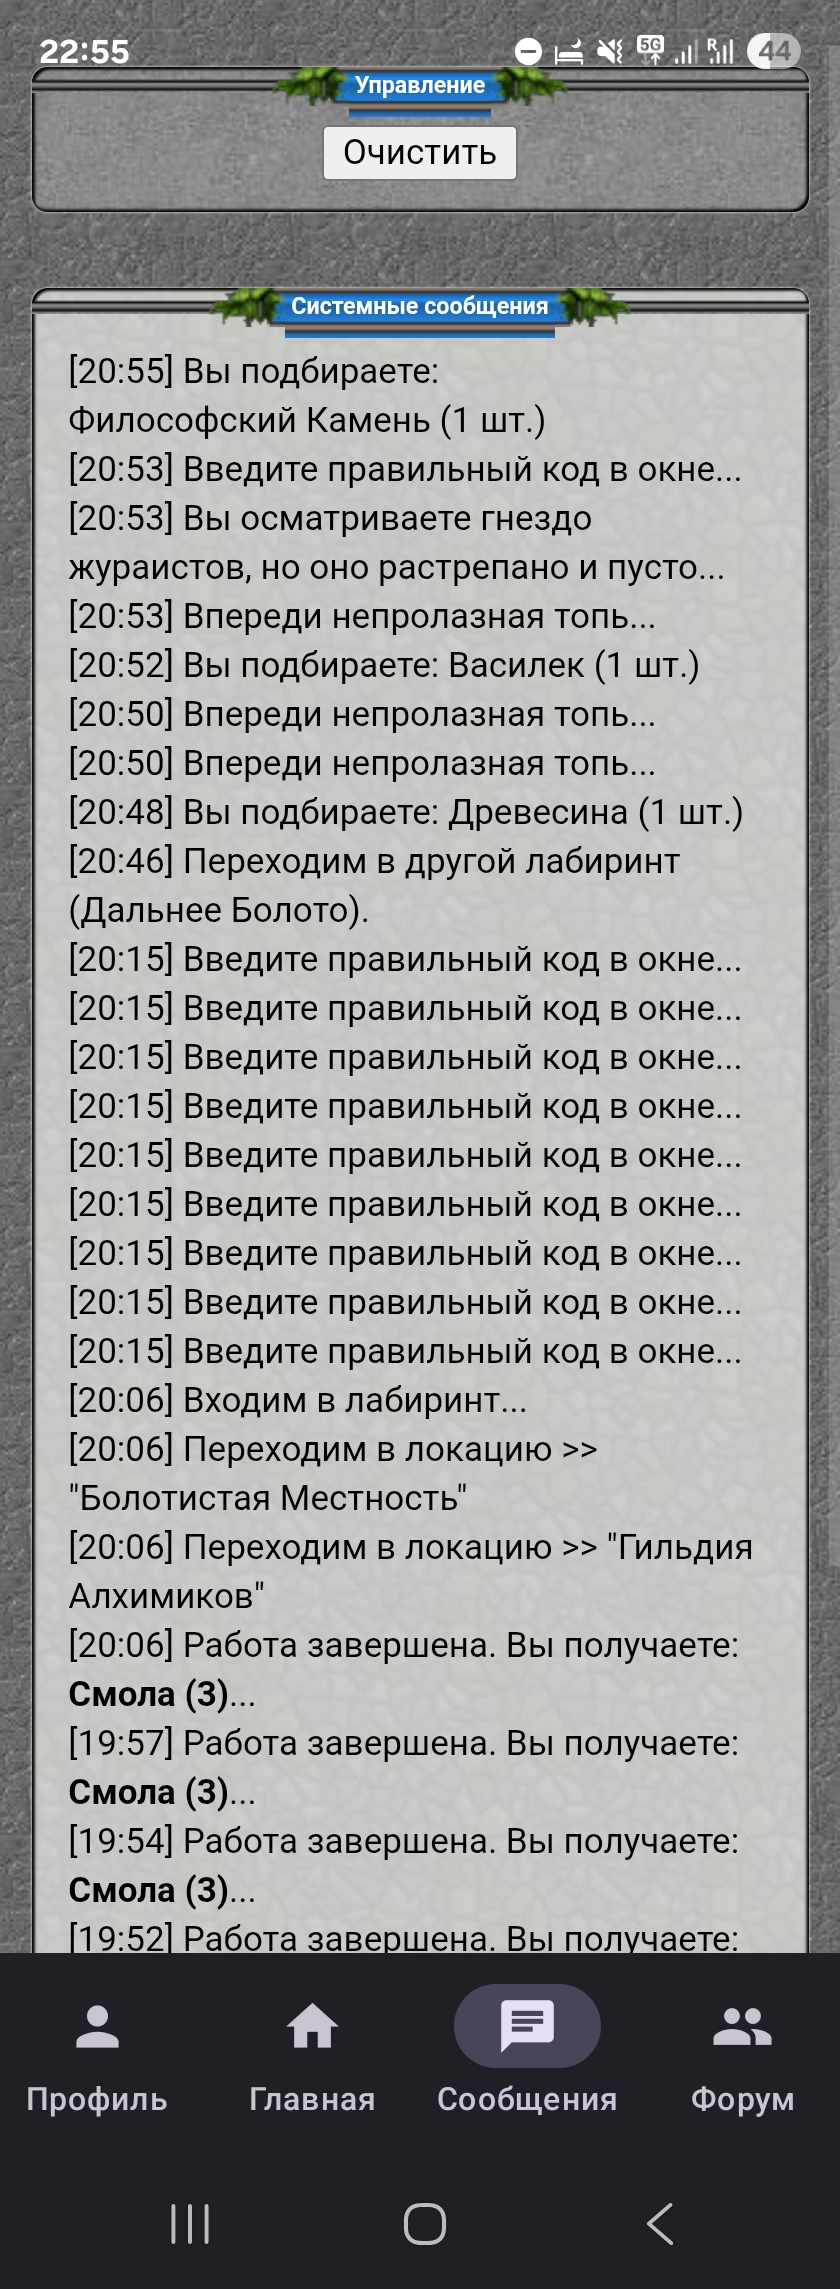
\includegraphics[width=0.24\textwidth]{../design-flow/chat_2.jpg}
  \caption{Concept of the application: login, movements, fight, and chat}
  \label{img:concept}
\end{figure}


\subsection{Shaping the Concept}
\markboth{Conceptualizing}{Shaping the Concept}

The application does not reimplement the game. Rather, it is an adapter between the player and
the game server. It must adhere to a few principles.

\begin{itemize}
  \item \textbf{Server is the source of truth} -- every action (a step in a labyrinth, a hit in
  a fight, a purchase in a tent) is forwarded to the server, and the application only shows the
  result. No game logic is duplicated, so the client cannot fall out of sync with the rules.

  \item \textbf{Progressive adaptation} -- the most used screens (main page, map, fights,
  labyrinths, chat, forum, tents) are parsed into data and rendered by mobile templates. Any
  other page is shown as is, with fixed links and images, so the player is never stuck at a
  missing screen.

  \item \textbf{Thumb-friendly navigation} -- the main sections (Profile, Home, Chat, Forum) are
  placed into a native tab bar at the bottom of the screen, while the content is drawn in a
  WebView above it.

  \item \textbf{Staying informed} -- chat messages and system events are delivered in the
  background and shown as toasts, and the screen is kept awake while the game is open.

  \item \textbf{Marketplace compliance} -- the client adds what stores demand from social
  applications: age assurance with parental restrictions, and account deletion from within the
  application.
\end{itemize}

\noindent The heart of the concept is \emph{URL mirroring}. The application registers the same
paths as the game server, so links inside a received page lead back to our controllers without
any rewriting:

\begin{lstlisting}
// routes/web.php
Route::get('/cgi/forum_rooms.php',
    [ForumController::class, 'index']);
Route::get('/cgi/maze_move.php',
    [LabController::class, 'move']);
// ... about a hundred routes

// All other routes
Route::get('/{any}',
    [GenericController::class, 'index'])
    ->where('any', '.*');
Route::post('/{any}',
    [GenericController::class, 'indexPost'])
    ->where('any', '.*');
\end{lstlisting}

\noindent Each request then travels through the same pipeline: a controller calls the game server
via \q{AppProxyProvider} (cURL with a cookie jar kept in the local storage), a parser extracts
the needed data from the received HTML, and a Blade template renders a mobile page:

\begin{figure}[h]
  \centering
  \begin{tikzpicture}[
      box/.style={draw, rounded corners, fill=backcolour, minimum height=0.8cm,
        align=center, font=\footnotesize},
      arr/.style={->, thick, codegray}]
    \node[box] (web) at (0,0) {WebView};
    \node[box] (ctrl) at (2.6,0) {Controller};
    \node[box] (proxy) at (5.4,0) {AppProxy\\(cURL)};
    \node[box] (srv) at (5.4,-1.8) {fantasyland.ru};
    \node[box] (parse) at (2.6,-1.8) {Parser};
    \node[box] (blade) at (0,-1.8) {Blade};
    \draw[arr] (web) -- (ctrl);
    \draw[arr] (ctrl) -- (proxy);
    \draw[arr] (proxy) -- (srv);
    \draw[arr] (srv) -- (parse);
    \draw[arr] (parse) -- (blade);
    \draw[arr] (blade) -- (web);
  \end{tikzpicture}
  \caption{Request pipeline inside the device}
  \label{img:concept-pipeline}
\end{figure}


\subsection{Choosing NativePHP}
\markboth{Conceptualizing}{Choosing NativePHP}

The nature of the task defines the necessary tools. Our application primarily converts one HTML
file into another. It sends forms, stores cookies, converts encodings, and extracts data using
regular expressions. These are daily routines for PHP, which has processed web pages since its
first release. Here's why NativePHP fits this concept especially well:

\begin{itemize}
  \item \textbf{No intermediate server} -- PHP runs on the device itself, so requests go from the
  player's phone directly to the game server. We don't need to host, scale, and pay for a proxy,
  and players' credentials and cookies never leave their devices.

  \item \textbf{No cross-origin limits} -- a JavaScript client inside a WebView (Cordova,
  Capacitor) cannot read responses from \q{fantasyland.ru} unless the server allows it by CORS
  headers, which we don't control. The embedded PHP makes plain HTTP calls with cURL and has no
  such restriction.

  \item \textbf{Familiar stack} -- routing, middleware, validation, queues, cache, and tests are
  the same as in any Laravel project (\cref{laravel}). Unparsed pages are passed to the WebView
  with minimal fixes, which lets the client grow screen by screen.

  \item \textbf{Native where it matters} -- the tab bar, toasts, and keeping the screen awake
  are provided by the native layer (\cref{nativephp}), while the rest of the interface stays in
  HTML and CSS.

  \item \textbf{One codebase, two platforms} -- the same PHP code is packaged for Android and
  iOS.
\end{itemize}

\noindent Alternatives were also considered. One option would be to create a wrapper around the
original website to maintain the desktop layout. A hosted Laravel proxy with a thin mobile
client would also work, but it would centralize all players' traffic and credentials on our
server. Using Flutter, Kotlin, or Swift would require rewriting all parsers in another language
(twice, in the case of separate native applications).


\newpage
\subsection{Weighing Pros and Cons}
\markboth{Conceptualizing}{Weighing Pros and Cons}

No technology is a silver bullet, and NativePHP brings its own trade-offs:

\begin{table}[!ht]
  \centering
  \footnotesize
  \begin{tabularx}{\textwidth}{|X|X|}
    \hline
    \textbf{Pros} & \textbf{Cons} \\
    \hline
    PHP and Laravel knowledge is reused; there's no need to learn Kotlin, Swift, or Dart &
    The bundle is heavy: the PHP runtime, Laravel, and \q{vendor} are packed into the build
    (our release \q{.aab} is about 68 MB) \\
    \hline
    One codebase for Android and iOS, with web-based interface that is already familiar &
    PHP sources are shipped as they are; Android minification and obfuscation apply only to the
    Kotlin/Java part, so secrets must be removed from the bundle \\
    \hline
    Works without own backend: the logic runs on the device &
    The first launch extracts the Laravel archive into the storage, and each WebView request
    boots the framework again \\
    \hline
    Native elements and device APIs are available through Laravel facades &
    The ecosystem is young: there are fewer plugins, and breaking changes between major
    versions are expected \\
    \hline
    Laravel testing (PHPUnit, Pest, fakes) covers most of the code without a device &
    Debugging spans three layers (PHP, WebView, Kotlin/Swift), and we had to patch the native
    project during the first startup \\
    \hline
    Open-source (MIT) core with an explicit plugin allow-list &
    Precompiled PHP binaries target \q{arm64-v8a}, so \q{x86\_64} emulators can't run builds,
    and iOS still requires macOS with Xcode \\
    \hline
  \end{tabularx}
  \caption{Pros and cons of NativePHP for the project}
  \label{tbl:concept-pros-cons}
\end{table}

\noindent For our concept, the advantages outweigh the drawbacks. The application is a thin
adapter on top of an existing web service. The hard part is parsing and adapting HTML, not
drawing complex animations or processing heavy graphics. The size of the bundle is the cost of
the embedded runtime. The young ecosystem is balanced by our ability to fix or extend the native
layer ourselves. In the following chapters, we will prepare the environment, solve the initial
startup issues, and transform this concept into a functioning application.
